\documentclass{article}

\usepackage{geometry}
\geometry{margin=2cm}
\usepackage{graphicx}
\usepackage{hyperref}
\usepackage{amsfonts}
\usepackage{caption}
\usepackage{subcaption}

\hypersetup{colorlinks=true, linkcolor=blue, urlcolor=blue}
\urlstyle{same}
\begin{document}
	
	\author{Aayush Arya}
	\date{(Submitted: \today)}
	\title{}
	
	\maketitle
	
	\hrule
	\begin{center}
		PHY366 Lab Report\\
		Practical: 8 \quad Registration No.: 11912610 \quad Section: G2903
	\end{center}
	\hrule
	
	\section*{Aim}
	To construct a modulator circuit using a transistor
	
	\section*{Methods}
	
	An amplitude modulation circuit was constructed using a transistor element. The circuit is available at \url{https://www.multisim.com/content/KEnsCE4LaBc7W8WNh3ZaY2/modulator-circuit/open/} and is shown in Figure \ref{fig:circuit}.
	
	\begin{figure}[!h]
		\centering
		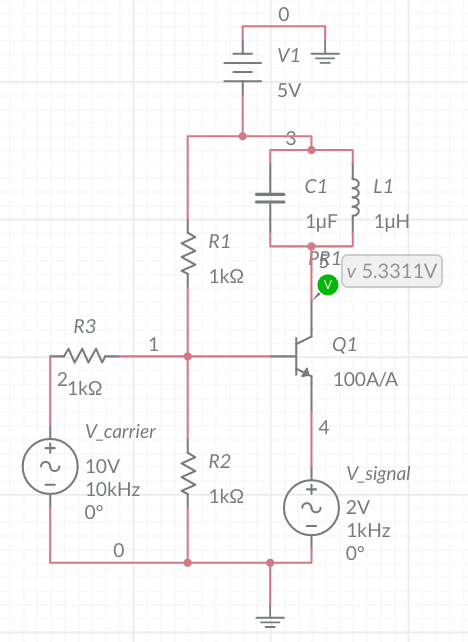
\includegraphics[width=0.5\textwidth]{circuit}
		\caption{Circuit diagram of the modulator}
		\label{fig:circuit}
	\end{figure}

	The signal $A_{signal}$ and $f_{signal}$ were kept fixed at 2V and 1 kHz respectively.
	
	\section*{Results \& Conclusions}
	We calculated the modulation index $$m = \frac{V_{max} - V_{min}}{V_{max} + V_{min}}$$ for each configuration studied.
	
	In Figure \ref{fig:example}, we show what the modulated signal output looks like, for an input carrier $A_c = 10V$ of frequency $f_c = 10$ kHz.
	
	\begin{figure}[h!]
		\centering
		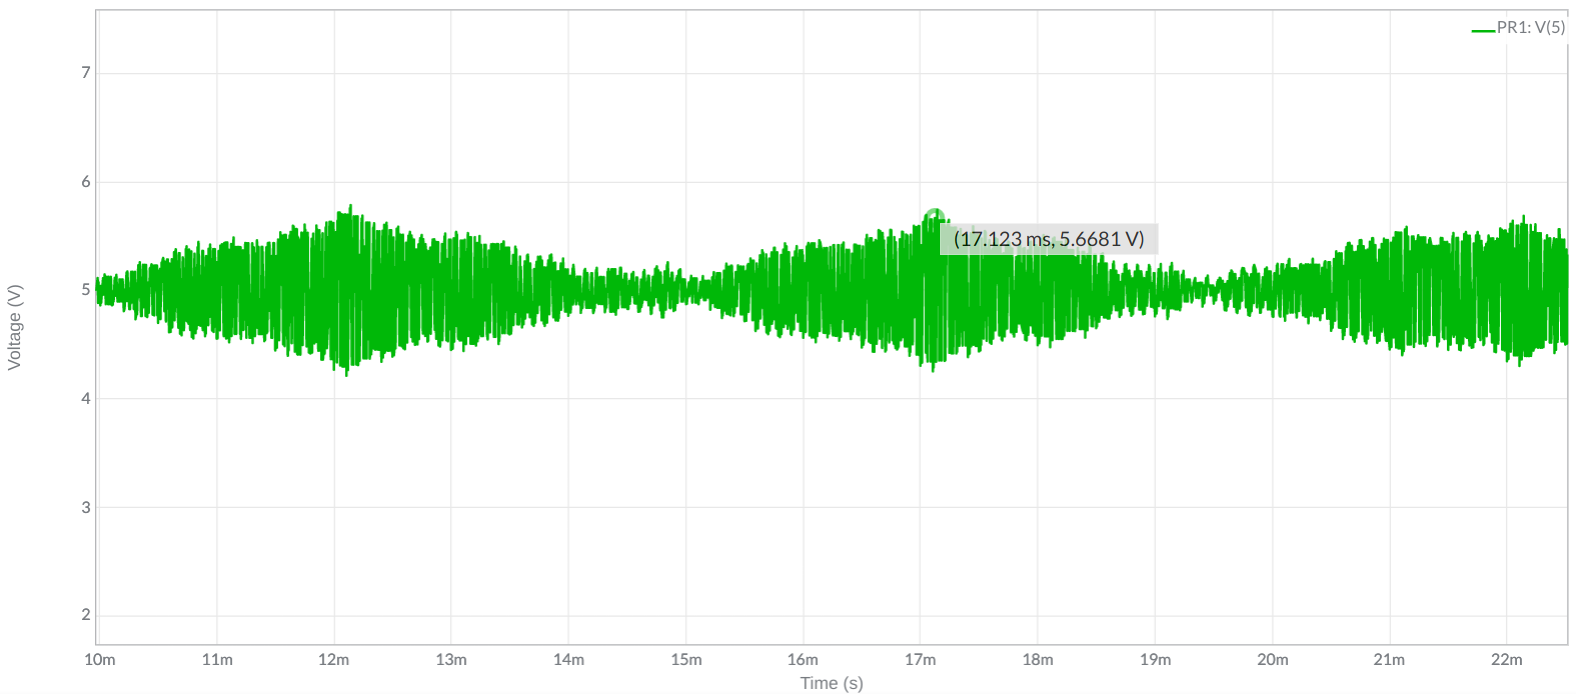
\includegraphics[width=0.8\textwidth]{example_mod}
		\caption{Modulated output signal for carrier $f_{c} = 10$ kHz and $A_c = 10$V.}
		\label{fig:example}
	\end{figure}

	By varying $f_c$ and $A_c$, we obtain the following $V_{max}$ and $V_{min}$ values.
	
	\begin{table}[!h]
		\centering
		\begin{tabular}{|c|c|c|c|c|}
			\hline
			$V_{max}  $           & $V_{min}$              & $f_c$ (kHz) 
			& $A_c$ (V) & $m$                   \\
			\hline
			0.6681 & 0.0744 & 10         & 10       & 0.7994  \\
			0.6821 & 0.1152 & 10         & 15       & 0.7110  \\
			1.7676 & 0.9980  & 100        & 10       & 0.2783 \\
			2.6944             & 1.7005              & 100        & 15       & 0.2261\\
			\hline
		\end{tabular}
		\caption{Summary of the measurements}
		\label{table}
	\end{table}

Note that since the $V_{CC}$ was kept at $5V$ DC, we subtracted this continuum value to obtain the correct $V_{max}$ and $V_{min}$\\ \noindent

Clearly, from Table \ref{table}, it's evident that the modulation index is larger for lower frequency and carrier amplitude.
 
\end{document}